%%----------------------------------------------------------------------------
%% Presentatie HoGent Bedrijf en Organisatie
%%----------------------------------------------------------------------------
%% Auteur: Bert Van Vreckem [bert.vanvreckem@hogent.be]

\documentclass{beamer}

%==============================================================================
% Aanloop
%==============================================================================

%---------- Packages ----------------------------------------------------------

\usepackage{graphicx,multicol}
\usepackage{comment,enumerate,hyperref}
\usepackage{amsmath,amsfonts,amssymb}
\usepackage{tikz}
\usepackage[dutch]{babel}
\usepackage[utf8]{inputenc}
\usepackage{multirow}
\usepackage{eurosym}
\usepackage{listings}
\usepackage[T1]{fontenc}
\usepackage{lmodern}
\usepackage{textcomp}
\usepackage{framed}
\usepackage{wrapfig}
%% voor grieks
%\usepackage[LGR,T1]{fontenc}
%\newcommand{\textgreek}[1]{\begingroup\fontencoding{LGR}\selectfont#1\endgroup}

%---------- Configuratie ------------------------------------------------------

\usetikzlibrary{arrows,shapes,backgrounds,positioning,shadows}

\usetheme{hogent}

%---------- Commando-definities -----------------------------------------------

\newcommand{\tabitem}{~~\llap{\textbullet}~~}

%---------- Info over de presentatie ------------------------------------------

\title[Intro]{Coding For Dummies}
\author{Jens {Buysse} / Stijn Lievens}
\date{\today}

%==============================================================================
% Inhoud presentatie
%==============================================================================

\begin{document}

%---------- Front matter ------------------------------------------------------

% Dia met het HoGent logo
\HoGentLogo

% Titeldia met faculteitslogo
\titleframe

%---------- Inhoud ------------------------------------------------------------

\begin{frame}
  \frametitle{Inhoud}

  \tableofcontents
\end{frame}


\section{De eerste codes}
\sectionframe{When Cryptography is outlawed, bayl bhgynjf jvyy unir cevinpl \\\begin{flushright}
		-- John Perry Barlow
\end{flushright} }

%% When cryptography is outlawed, only outlaws will have privacy.

\begin{frame}{Cryptografie}
	Het woord \textcolor{HoGentBlue}{cryptografie} betekent letterlijk  \textcolor{HoGentBlue}{‘geheim schrijven’} of  \textcolor{HoGentBlue}{‘verborgen schrijven’}.\\
	We herkennen hierin de 2 Griekse woorden 
	\begin{itemize}
		\item kruptos  en %$\kappa \rho \upsilon \pi \tau \omicron \sigma $ (\textgreek{kruptos)}
		\item graphein
	\end{itemize}
	 wat samen ‘geheim schrijven’ betekent.
\end{frame}

\begin{frame}{De eerste codes}
	Zowel de Romeinen als de Grieken verdiepten zich in de grondbeginselen van cryptografie. 
	
	\begin{itemize}
		\item Optische signalen m.b.h.v. toortsen
		\item vlaggen
		\item spiegels
		\item \dots
	\end{itemize}
\end{frame}

\begin{frame}{De eerste codes}
	\begin{figure}
		
\includegraphics[width=\textwidth]{img/toorts.jpg}
	\end{figure}
\end{frame}


%% Aeanas: 4e eeuw BC


\begin{frame}{Aenas' Telegraaf}
\begin{figure}
	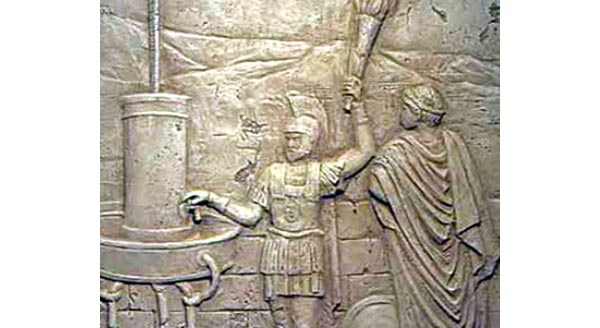
\includegraphics[width=\textwidth]{img/aenas.jpg}
\end{figure}
\end{frame}

\begin{frame}{Aenas' Telegraaf}
\begin{enumerate}
\item Partij A heft een brandende fakkel
\item Partij B heft ten antwoord ook een brandende fakkel
\item Partij A laat fakkel zaken en kranen worden open gezet
\item Partij A heft opnieuw brandende fakkel op zodat kranen gesloten kunnen worden.
\item Stand van het water duidt de verzonden boodschap aan.
\end{enumerate}

\pause 
Nadeel: Slechts een beperkt aantal boodschappen kon verzonden worden.
\end{frame}


% Polybius:  c. 200 – c. 118 BC


\begin{frame}{Polybius}
	Code ontwikkeld door Griekse militair.
	\[ \begin{bmatrix}
		  & 1  & 2  & 3  & 4  & 5\\ 
		1 & A  & B  & C  & D  & E\\ 
		2 & F  & G  & H  & I  & J \\ 
		3 & K  & L  & M  & N  & O \\ 
		4 & P  & Q  & R  & S  & T\\ 
		5 & V  & W  & X  & Y  & Z  
	\end{bmatrix}  \]
	
	\pause Merk op: er is geen apart teken voor U (identiek aan V)
	
	\pause
	Wat betekent volgend geheimschrift?
	\[ \begin{bmatrix}
12 & 53 & 34 & 54 & 15 & 43 & 51 & 12 & 11 & 15 \\ 
53 & 34 & 44 & 54 & 32 & 51 & 21 & 53 &23 &41 
\end{bmatrix} \]
\end{frame}

%% Antwoord. FORTUNEFAVORSTHEBOLD
%% Dit is een uitspraak van Scipio Africanus

\begin{frame}{Polybius}
	Er werden twee reeksen van fakkels opgesteld:
	\begin{enumerate}
		\item Eerste 5 fakkels duiden de kolom aan
		\item Tweede 5 fakkels duiden de rij aan
	\end{enumerate}
    
    \pause
    Hoe snel is dit systeem?\pause
    
    Antwoord: studenten uit Aken in jaren '80: 8 letters/minuut.\pause
    Als 1 letter gelijk is aan 8 bits: 64 bits/minuut
    
\end{frame}


%% Caesar: eerste eeuw voor christus (55BC : De Bello Gallico)

\begin{frame}[fragile]{Caesarscode}
	Elke letter wordt vervangen door de letter die een afgesproken aantal plaatsen (bv.\ 3) verder in het alfabet staat. 
	
	\begin{center}
		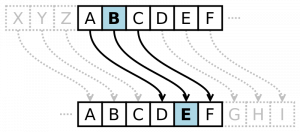
\includegraphics[width=0.5\textwidth]{img/Caesar-Code.png}
	\end{center}
	
	
	Na de 'Z' komt opnieuw de 'A'.
	
	\begin{block}{Code}
	EDG LV D SODQ ZKLFK FDQQRW EHDU D FKDQJH
	\end{block}
\end{frame}

%% Antwoord: BAD IS A PLAN WHICH CANNOT BEAR A CHANGE


\begin{frame}[fragile]{Caesarscode - zwaktes}
	Wat zijn de zwaktes van deze codering en hoe zou je deze aanpakken?
	\pause
	\begin{itemize}
		\item Biedt slechts 25 mogelijkheden tot versleuteling. (Computer kan dit makkelijk kraken)
		\item De letter 'E' komt heel erg vaak voor in de taal. 
		Door te tellen welke letter het meest voorkomt kan je al goed raden wat de E zal zijn. 
		\item Je weet ook al wat de woorden zijn.
	\end{itemize}

\begin{center}
\begin{block}{Code}
ROHXD VDBCK ANJTC QNUJF MXRCC XBNRI
NYXFN ARWJU UXCQN ALJBN BXKBN AENRC
\end{block}
\end{center}
\end{frame}

%% Antwoord: IFYOU MUSTB REAKT HELAW DOITT OSEIZ EPOWE RINAL LOTHE RCASE SOBSE RVEIT

%% Deze code kan gemakkelijk "gekraakt" worden. De meest voorkomende letter is 'N'.  'N' - 'E' = 9. 
%% Dus proberen te decoderen met shift = 9.


%% Scytale: ontwikkeld in de 7de eeuw voor Christus.
%% Scytale is eeen voorbeeld van een transpositiecijfer: de tekens worden van plaats gewisseld
%% De dikte van het cilindrisch voorwerp is de 'sleutel'.

\begin{frame}[fragile]{Scytale}
	\begin{figure}
		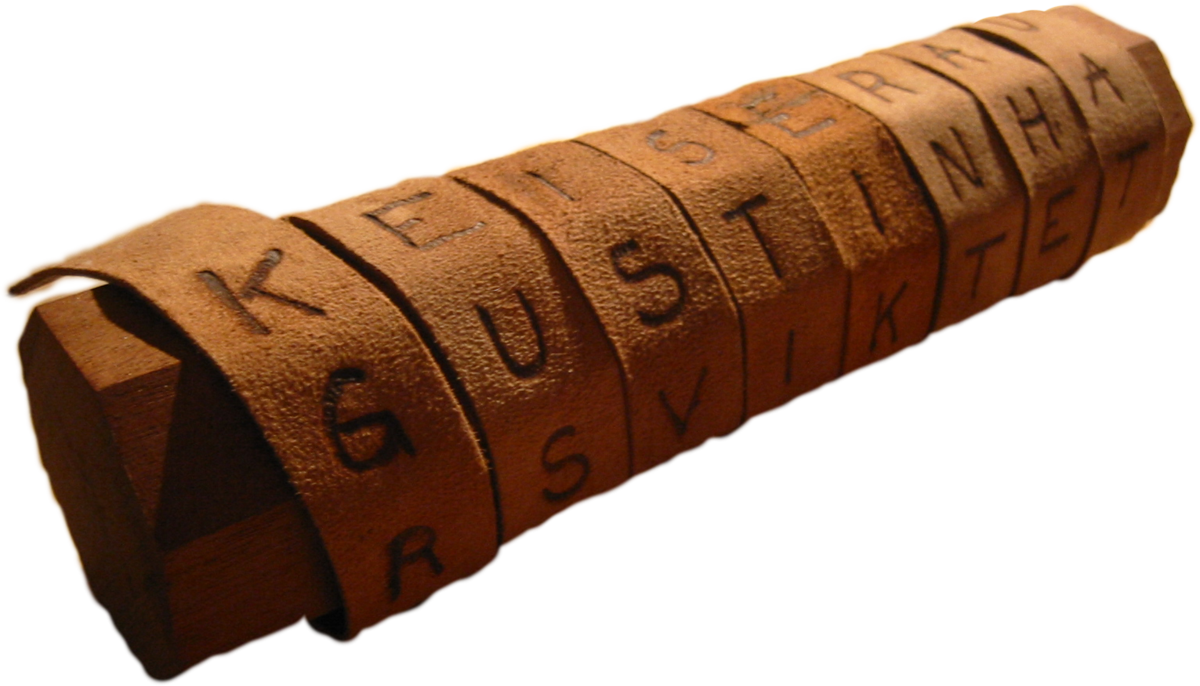
\includegraphics[width=\textwidth]{img/scytale}
	\end{figure}

\begin{block}{Code}
	ANACD DEIOR SUTWB AOTIR FNSUE ELNTF EHRMA IYNE
\end{block}
\end{frame}

%% Lees elke derde letter. Start bij derde/tweede/eerste letter.
%% Spaties worden genegeerd.
%% Antwoord: A DOUBTFUL FRIEND IS WORSE THAN A CERTAIN ENEMY

\section{Iets formeler}
\sectionframe{Cryptography shifts the balance of power from those with a monopoly on violence to those who comprehend mathematics and security design. \\\begin{flushright}
		Jacob Appelbaum
\end{flushright}}

%% Bij cryptography is de assumptie dat Eve alles kan horen wat er tussen Alice en Bob
%% wordt gezegd. Zij mag niet (of heel moeilijk) in staat zijn om uit te vissen wat er 
%% tussen Alice an Bob wordt gezegd.  M.a.w. ze mag niets leren over de inhoud van de
%% plaintext.

\begin{frame}{Alice, Bob \& Eve}
	\begin{figure}
		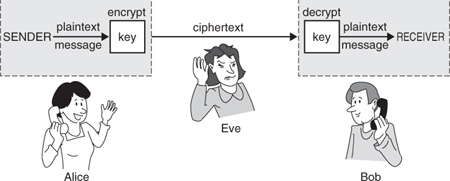
\includegraphics[width=\textwidth]{img/adameve.jpg}
	\end{figure}
\end{frame}

\begin{frame}{Cryptografieindeling}
	\begin{description}
		\item[Symmetrisch] Wanneer de sleutel om te versleutelen en ontsleutelen dezelfde is. Versleuteling kan enkel veilig gebeuren wanneer er een veilige sleuteluitwisseling tussen Alice en Bob gebeurd is.
	\item[Asymmetrisch] Of ook \textbf{publieke sleutel} cryptografie waarbij het versleutelen en ontsleutelen met een verschillende sleutel moet
	gebeuren.
\end{description}
We merken op dat hedendaagse versleutelingsmechanismen vaak een gelaagde combinatie van bovengenoemde types zijn.
\end{frame}

\begin{frame}{Symmetrische vs Asymmetrische Encryptie}
\begin{figure}
	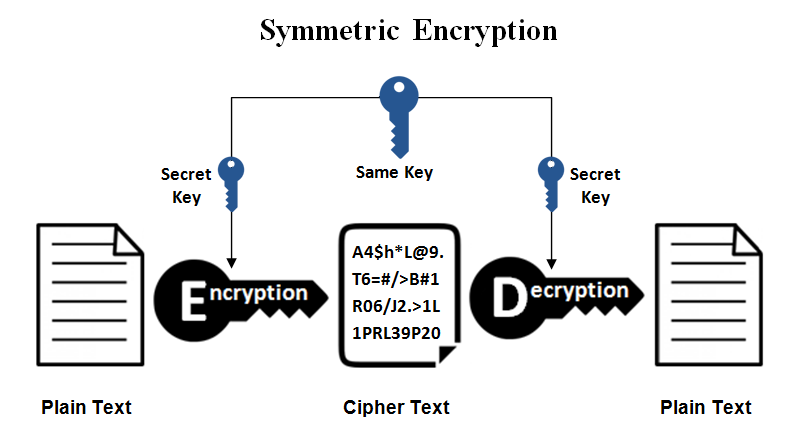
\includegraphics[width=0.50\textwidth]{img/Symmetric-Encryption.png}
	\quad
	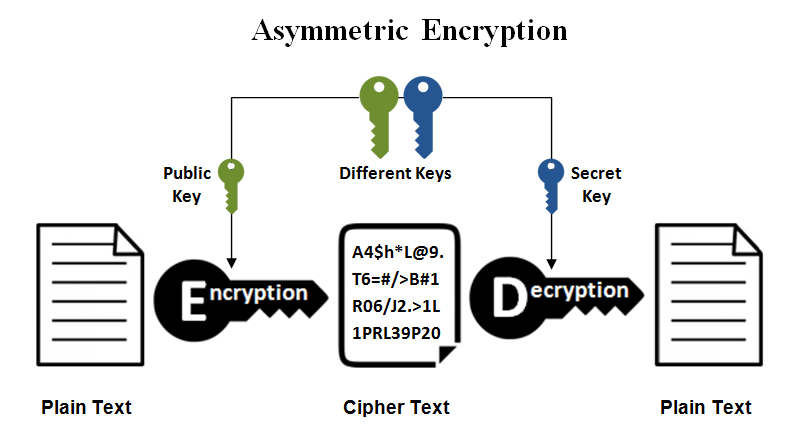
\includegraphics[width=0.50\textwidth]{img/Asymmetric-Encryption.png}
\end{figure}
\end{frame}

\begin{frame}{Enkele definities}
	\begin{description}
		\item[Plaintext / Cleartext] Het ongecodeerde bericht. 
			
		\item[Encryption] Het proces van het coderen van de plaintext.
		\item[Ciphertext] 
		
		Dit is de uiteindelijke tekst, in versleutelde vorm. Bij een goed gecodeerde tekst is de ciphertext een onbegrijpelijke boodschap, waaruit onbevoegden praktisch onmogelijk de plaintext kunnen halen.
		\item[Decryption] 
		
		De decryption is de stap die de ontvanger uitvoert om het originele bericht weer uit de ciphertext te halen. 
		\item[Key] 
		
		De key is de sleutel die je nodig hebt om een ciphertext te decoderen. 
		\item[Cryptanalysis] 
		Dit begrip houdt het kraken van een gecodeerde tekst in. 
		\item[Cryptology] 
		Cryptologie is een net iets minder ruim begrip dan Cryptografie. Bij cryptologie wordt namelijk alleen de wiskundige kant van de cryptografie bestudeerd.
	\end{description}
\end{frame}

\begin{frame}{Voorbeeld Plaintext en Ciphertext}
\begin{center}
\begin{figure}
	
\includegraphics[width=0.40\textwidth]{img/tux.png}
	\quad
	
\includegraphics[width=0.40\textwidth]{img/tux_secure.png}
\end{figure}
\end{center}
\end{frame}



\begin{frame}{Voorbeeld Plaintext en Zwakke Ciphertext}
\begin{center}
	\begin{figure}
		
\includegraphics[width=0.40\textwidth]{img/tux.png}
		\quad
		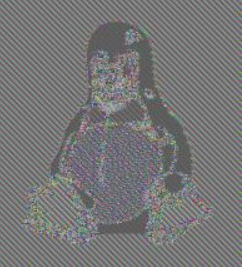
\includegraphics[width=0.40\textwidth]{img/tux_ecb.png}
	\end{figure}
\end{center}
\end{frame}


%% Auguste Kerchoffs: 1835 -- 1903. Nederlands taalkundige en cryptograaf. Was professor in Parijs aan het einde van de 19e eeuw.
%% De 6 principes werden in 1883 gepubliceerd in een Frans tijdschrift.

\begin{frame}{Kraakpogingen - Kerckhoffs' principes}
	
	\begin{enumerate}
		\item Het systeem dient, zelfs als het in theorie niet onbreekbaar is, in de praktijk onbreekbaar te zijn. \pause
		\item \textcolor{HoGentAccent1}{Het ontwerp van het systeem behoort \emph{niet} geheim te hoeven zijn en dient, indien gecompromitteerd, de correspondenten niet te kunnen schaden.}\pause
		\item De sleutel moet onthoudbaar zijn zonder notities en dient makkelijk veranderd te kunnen worden.\pause
		\item De cryptogrammen moeten overgebracht kunnen worden door middel van telegrafie.\pause
		\item Het apparaat of de documenten dienen draagbaar te zijn en te kunnen worden bediend door een enkel persoon.\pause
		\item Het systeem dient gemakkelijk te zijn, niet onderhevig aan kennis van allerlei regels of aan mentale inspanning\pause
\end{enumerate}
	\textcolor{HoGentAccent1}{Belangrijk: \textit{principe van Kerckhoffs}}: de veiligheid van een cryptografisch systeem mag \textbf{niet} van de geheimhouding van het \textbf{versleutelingssysteem} maar slechts van de geheimhouding van de \textbf{sleutel} afhangen.

\end{frame}

\begin{frame}{Kraakpoging - Brute Force}
	\brightbox{Brute force (Engels voor "brute kracht") is het gebruik van rekenkracht om een probleem
    op te lossen met een computer zonder gebruik te maken van algoritmen of heuristieken}

\begin{itemize}
	\item 	 De methode bestaat m.a.w.\ uit het botweg uitproberen van alle mogelijke mogelijkheden (sleutels), 
	 tot er een gevonden is die overeenkomt met de gewenste uitvoer.
\end{itemize}
\end{frame}

\begin{frame}{Combo Attack}
	Gebruik een woordenboek en plak de verschillende woorden tezamen.
	\begin{itemize}
		\item dictionary1.txt \& dictionary2.txt
		\item pass $ \rightarrow $ password, passpass, passlion
		\item word $ \rightarrow $ wordpass, wordword, wordlion
		\item lion $ \rightarrow $ lionpass, lionword, lionlion 
	\end{itemize}
\end{frame}

\begin{frame}{Combo Attack}
Combo attack, maar met de mogelijkheid een willekeurige reeks letters toe te voegen
	\begin{itemize}
	\item dictionary.txt \& abcde
	\item pass $ \rightarrow $ passAbc, passBcd, passCde
	\item word $ \rightarrow $ wordAbc, wordBcd, wordCde
	\item lion $ \rightarrow $ lionAbc, lionBcd, lionCde
	\end{itemize}
\end{frame}

%\begin{frame}{Use Case: Wordpress websites}
%	Als je gebruikmaakt van Wordpress ben je kwetsbaar voor Brute Force attacks.
%	
%	Je kan hiertegen een aantal eenvoudige maatregelen gebruiken:
%	\begin{enumerate}
%		\item Sterke paswoorden gebruiken
%		\item De admingebruikersnaam veranderen
%		\item Het aantal loginpogingen beperken
%		\item Loginpagina anders noemen
%		\item IP adressen die toegang hebben beperken
%		\item CAPTCHA toevoegen
%	\end{enumerate}
%\end{frame}


\section{RSA}
\sectionframe{\begin{center}
		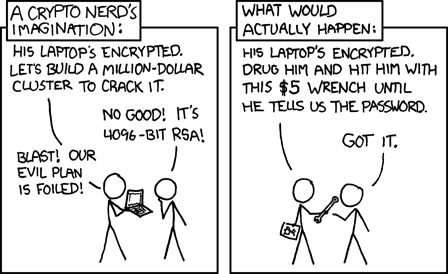
\includegraphics[width=\textwidth]{img/security.png}
\end{center}}


\begin{frame}{RSA}

\textbf{-----BEGIN PUBLIC KEY-----}\\
MIIBIjANBgkqhkiG9w0BAQEFAAOCAQ8AMIIBCgKCAQEAvUWEGue
PMihBxG8/mhi1z9YdCXEDk01iqLcYEKa4uPfPao0DAU2/4hSkWu
JCgBkAzJns8hz7DKskdRrTnhG1rcomyLFz07GFq1qkmpc6bL1UW
UNsdIOtu0CsgbtdeFW5OMJhezljf/jvuYRpE+eNPwHmg0233JvN
TVQ2ZNUO9eXX7gt1qYKZiHR3warYYE+7ro6BOwY3pBOG8iIm3zj
u2ioICGFH/hd9Jd19+mZwWneccYv89W1eSyPYg5yBWIIYLSFZA9
imlO0Xe3/ifRQyDjaE5YbTQt6/CkBYmObp009Exp3QwPnpYLTKM
zhjfgk+5Bg3O2wVVX+1ny7QqLSHrQIDAQAB\\
\textbf{-----END PUBLIC KEY-----}
\end{frame}

\begin{frame}{RSA}
	
\includegraphics[width=\textwidth]{img/secret.png}
\end{frame}

\begin{frame}{RSA}
	
\includegraphics[width=\textwidth]{img/bank.jpg}
\end{frame}

%\begin{frame}{RSA}
%	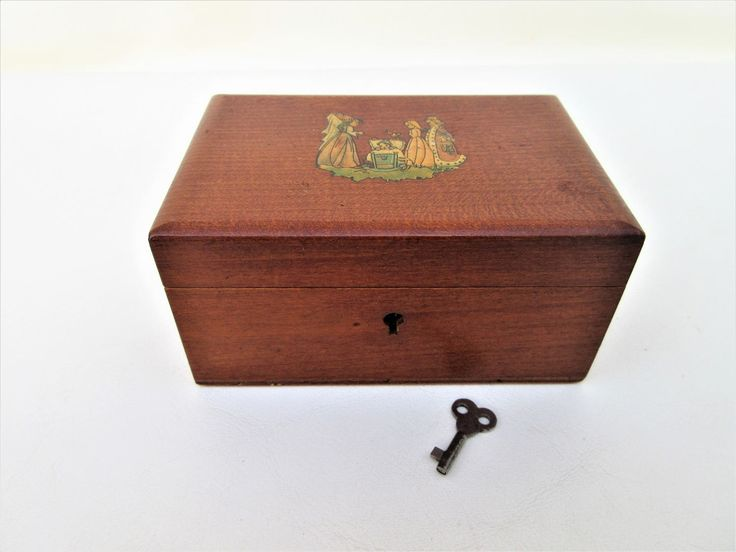
\includegraphics[width=\textwidth]{img/box.jpg}
%\end{frame}
%
%\begin{frame}{RSA}
%	\begin{columns}
%		\begin{column}[T]{0.5\textwidth}
%			
\includegraphics[width=\textwidth]{img/bank.jpg}
%		\end{column}
%	
%		\begin{column}[T]{0.5\textwidth}
%			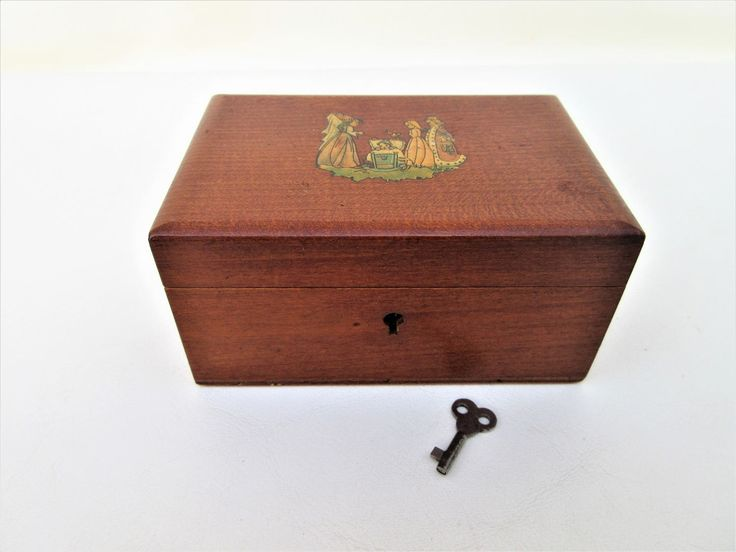
\includegraphics[width=0.3\textwidth]{img/box.jpg}
%			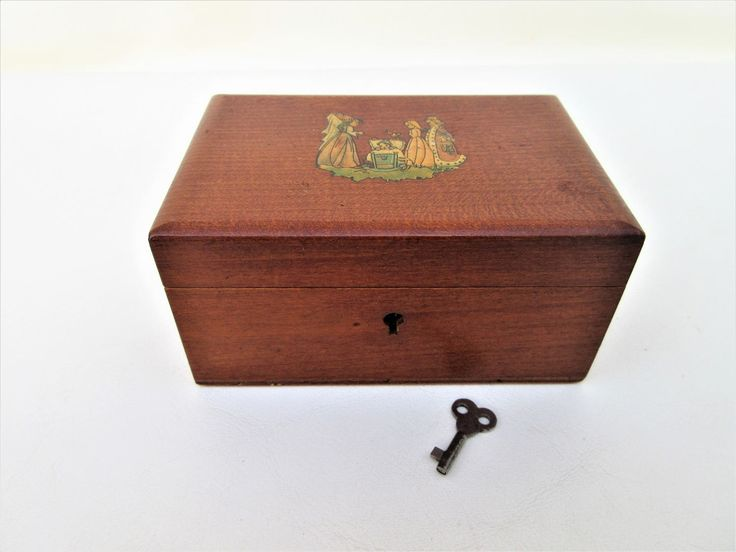
\includegraphics[width=0.3\textwidth]{img/box.jpg}
%			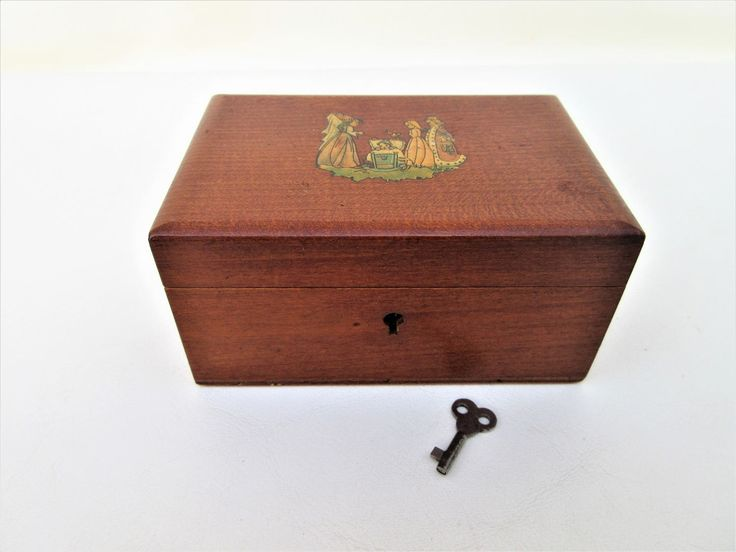
\includegraphics[width=0.3\textwidth]{img/box.jpg} \\
%						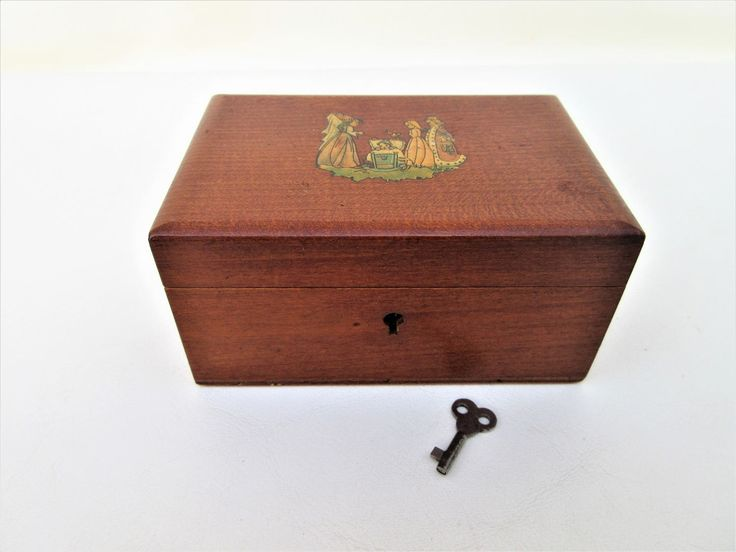
\includegraphics[width=0.3\textwidth]{img/box.jpg}
%			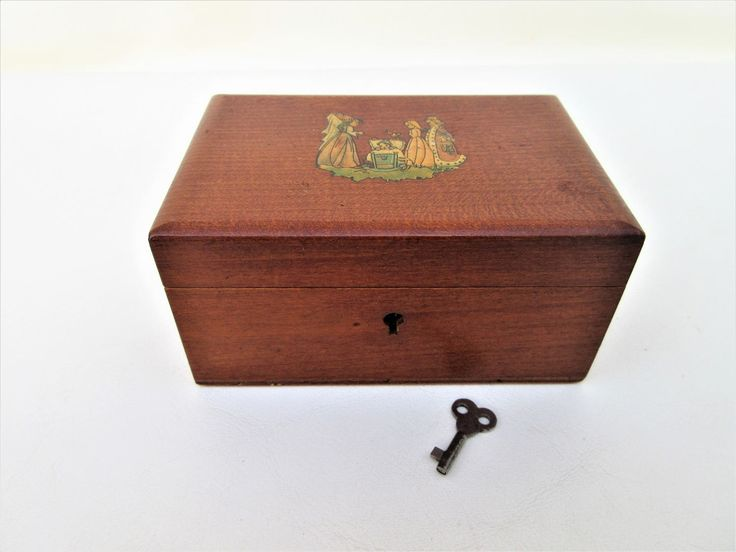
\includegraphics[width=0.3\textwidth]{img/box.jpg}
%			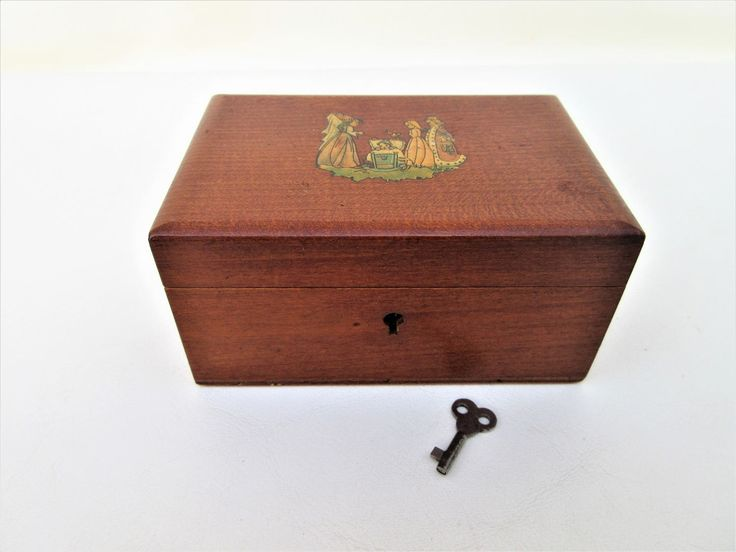
\includegraphics[width=0.3\textwidth]{img/box.jpg} \\
%						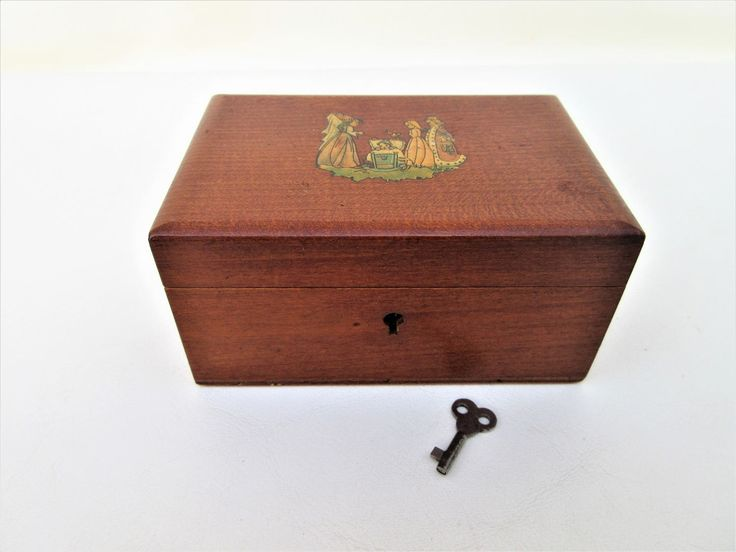
\includegraphics[width=0.3\textwidth]{img/box.jpg}
%			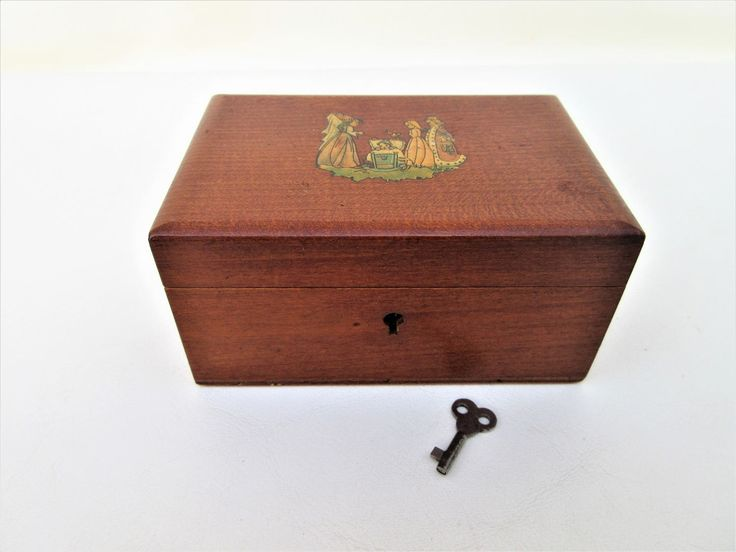
\includegraphics[width=0.3\textwidth]{img/box.jpg}
%			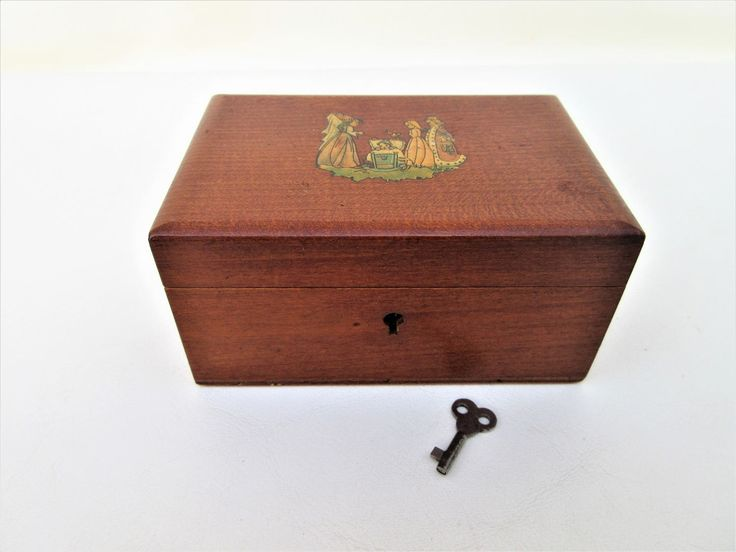
\includegraphics[width=0.3\textwidth]{img/box.jpg}
%		\end{column}
%	\end{columns}
%\end{frame}
%
%\begin{frame}{RSA}
%	\begin{center}
%		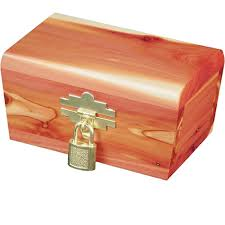
\includegraphics[width=0.4\textwidth]{img/padlock.jpeg}
%	\end{center}
%\end{frame}
%
%\begin{frame}{RSA}
%	\begin{columns}
%		\begin{column}[T]{0.5\textwidth}
%			
\includegraphics[width=\textwidth]{img/bank.jpg}
%		\end{column}
%		
%		\begin{column}[T]{0.5\textwidth}
%			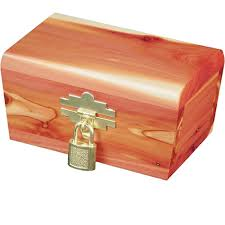
\includegraphics[width=0.3\textwidth]{img/padlock.jpeg}
%			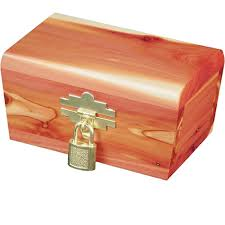
\includegraphics[width=0.3\textwidth]{img/padlock.jpeg}
%			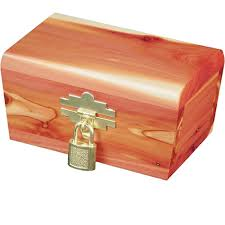
\includegraphics[width=0.3\textwidth]{img/padlock.jpeg} \\
%			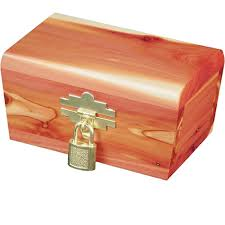
\includegraphics[width=0.3\textwidth]{img/padlock.jpeg}
%			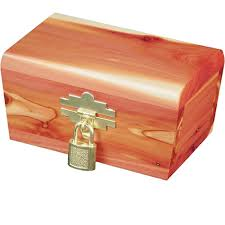
\includegraphics[width=0.3\textwidth]{img/padlock.jpeg}
%			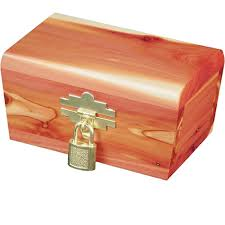
\includegraphics[width=0.3\textwidth]{img/padlock.jpeg} \\
%			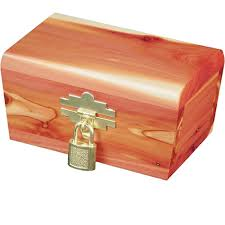
\includegraphics[width=0.3\textwidth]{img/padlock.jpeg}
%			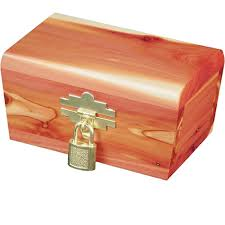
\includegraphics[width=0.3\textwidth]{img/padlock.jpeg}
%			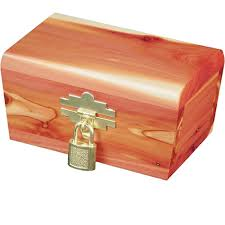
\includegraphics[width=0.3\textwidth]{img/padlock.jpeg}
%		\end{column}
%	\end{columns}
%\end{frame}

\subsection{Modulo rekenen}
\begin{frame}{Modulo rekenen}
	\begin{columns}
		\begin{column}[T]{0.5\textwidth}
			Stel dat het op een moment 20 uur is, en je telt daar 7 uur bij op. Dan zou het volgens gewone rekenmethodes dus 20 + 7 = 27 uur moeten zijn.
			
			Maar niemand noemt dat 27 uur, iedereen zegt 3 uur. Dat komt natuurlijk omdat het de volgende dag is geworden en die 24 uur van de vorige dag interesseren ons niet zoveel meer.
		\end{column}
		
		\begin{column}[T]{0.5\textwidth}
				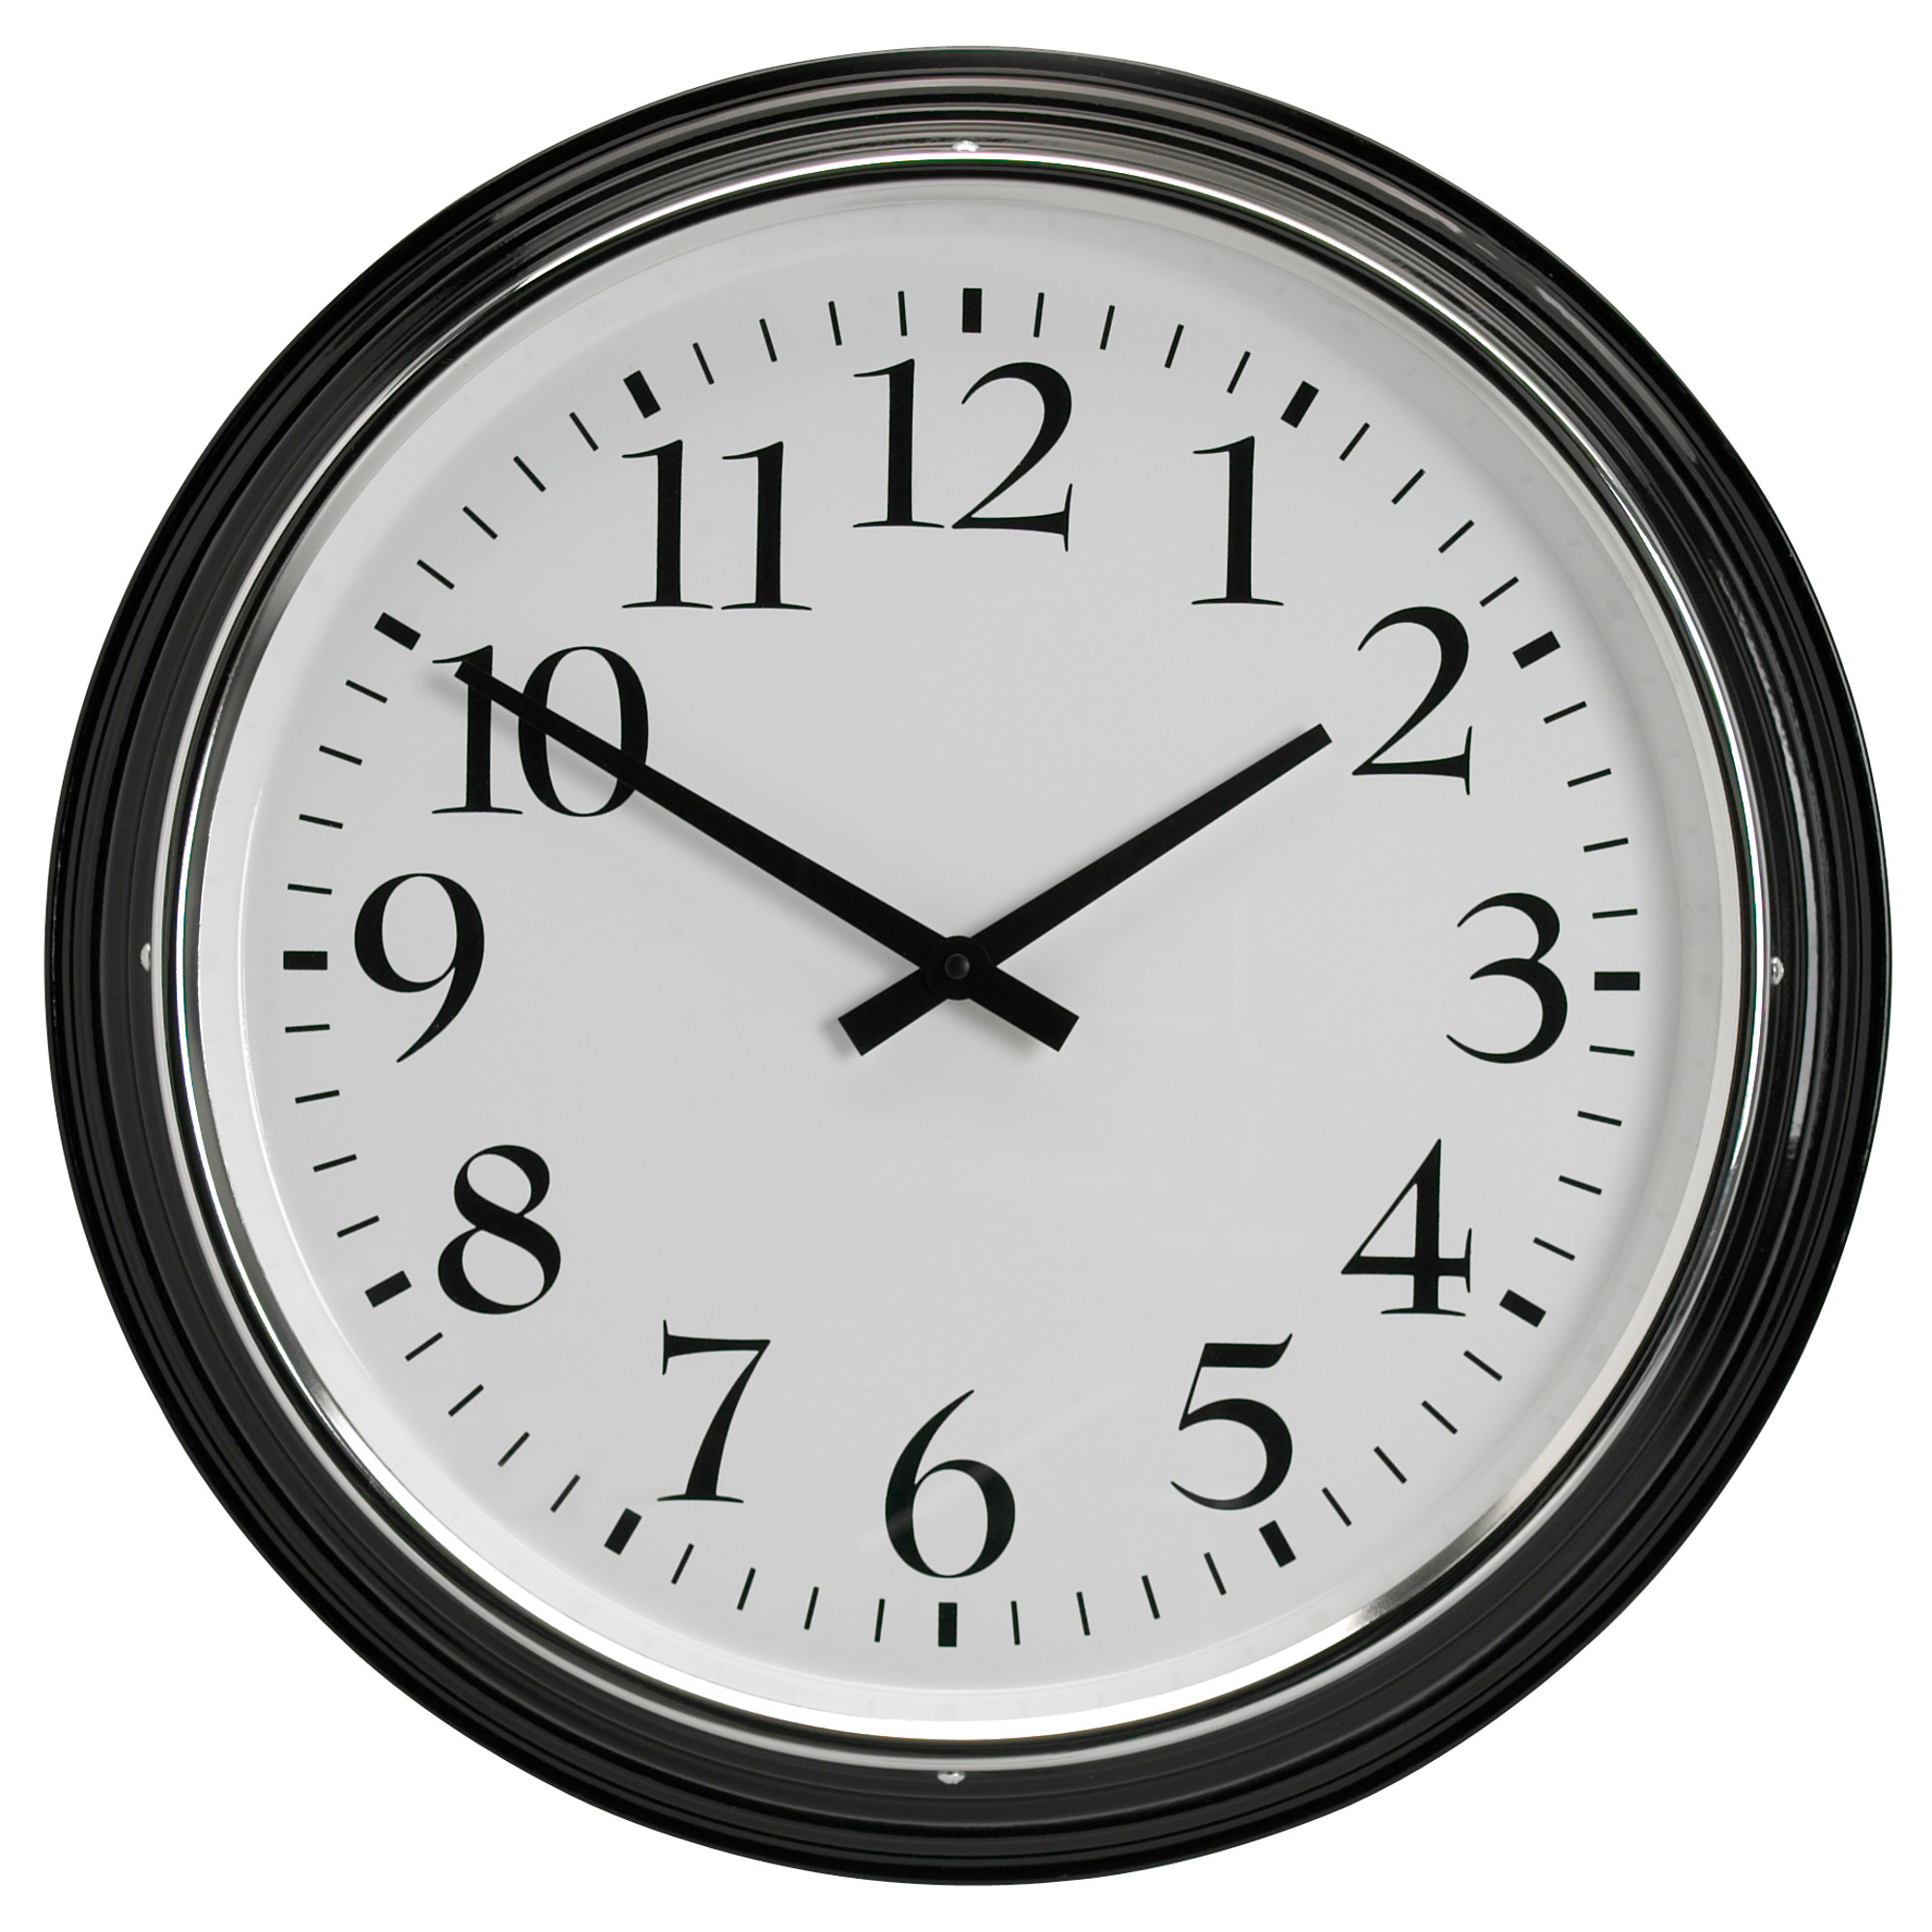
\includegraphics[width=\textwidth]{img/clock.jpg}
		\end{column}
	\end{columns}
\end{frame}

\begin{frame}{Modulo rekenen}

	Zij $n$ een natuurlijk getal $\neq 0$, dan heten de twee gehele getallen $a$ en $b$ \textbf{congruent} modulo $n$, genoteerd:
	\[ 
		a \equiv b \pmod{n}
	\]
	
	als hun verschil $a - b$ een geheel veelvoud is van $n$.
	
	Het getal $n$ wordt de \textbf{modulus} genoemd.
	
	We noteren 
	\[
	a \pmod{n} 
	\]
	als het getal tussen $0$ en $n-1$ waar $a$ congruent mee is modulo $n$.
	
\end{frame}

\begin{frame}{Voorbeelden modulo rekenen}
	\begin{eqnarray*}
			26  \pmod{8} &= \pause 2 \\
			-13 \pmod{8} &= \pause 3 \\
			257 \pmod{8} &= \pause 1 
	\end{eqnarray*}
\end{frame}

%\begin{frame}{Andere notatie}
%	\begin{eqnarray*}
%	26  \pmod{8} &=  2 + k \times 8 \\
%	-13 \pmod{8} &= 3 + k \times 8\\
%	257 \pmod{8} &=  1 + k \times 8
%	\end{eqnarray*}
%\end{frame}

\begin{frame}{Modulo Rekenregels: Optelling}
	\[ a \pmod{n} + b \pmod{n}  =  (a + b)  \pmod{n}\]
	
	\vspace{0.5cm}
	Voorbeeld: Stel $a = 23$, $b = -10$ en $n = 8$.
	\begin{itemize}
	\pause \item We berekenen het rechterlid: $a + b = 13$ zodat $13 \pmod 8 = 5$.
	\pause \item We berekenen het linkerlid:
	 \begin{itemize}
	   \pause\item $a \pmod n = 23 \pmod{8} = 7$
	   \pause\item $b \pmod n = -10\pmod{8} = 6$
	   \pause \item $7 + 6 = 13$ en $13 \pmod{8} = 5$ 
	\end{itemize}
	\end{itemize}
	
	
	 
\end{frame}

\begin{frame}{Modulo Rekenregels: Vermenigvuldiging}
	\[ a \pmod{n} \times b \pmod{n}  =  (a \times b)  \pmod{n}\]
		\vspace{0.5cm}
	Voorbeeld: Stel $a = 23$, $b = -10$ en $n = 8$.
	\begin{itemize}
		\pause \item We berekenen het rechterlid: $a \times b = -230$ zodat $-230 \pmod 8 = 2$ (want $-230 = - 29 \times 8 + 2)$
		\pause \item We berekenen het linkerlid:
		\begin{itemize}
			\pause\item $a \pmod n = 23 \pmod{8} = 7$
			\pause\item $b \pmod n = -10\pmod{8} = 6$
			\pause \item $7 \times 6 = 42$ en $42 \pmod{8} = 2$ 
		\end{itemize}
	\end{itemize}
\end{frame}

\begin{frame}{Modulo Rekenregels: Machtsverheffing}
	\[ (a \pmod{n})^m  =  a^m  \pmod{n}\]
	\vspace{0.5cm}
	Voorbeeld: Stel $a = 23$, $m = 5$ en $n = 8$.
		\begin{itemize}
		\pause \item We berekenen het rechterlid: $23^5 = 6436343$ zodat $6436343 \pmod 8 = 7$ 
		(want $6436343 = 804542 \times 8 + 7)$
		\pause \item We berekenen het linkerlid:
		\begin{itemize}
			\pause\item $a \pmod n = 23 \pmod{8} = 7$
			\pause\item $7^5 = 16807$
			\pause \item $16807 \pmod{8} = 7$ (want $16807 =2100 \times 8 + 7$)
		\end{itemize}
	\end{itemize}
	
\end{frame}

\begin{frame}{Toepassing bankrekeningen - Nederland}
Een rekeningnummer bestaat uit 9 cijfers:
	\[ c_9c_8c_7c_6c_5c_4c_3c_2c_1\]
	
Een rekeningnummer is \textbf{geldig} wanneer:
\[
9\times c_9 + 8\times c_8 + 7\times c_7 + \cdots + 2\times c_2 + c_1 \equiv 0 \pmod{11}.
\]	
	
M.a.w.\ de som die berekend wordt moet steeds een veelvoud zijn van 11.
\end{frame}

\begin{frame}{Toepassing bankrekeningen - Nederland}
	\[ 45824365c_1\]
	bepaal
	\begin{align*}
& 	 9 \times 4 + 8 \times 5 + 7\times 8 + 6\times 2 + 5\times 4 + 4\times 3 + 3\times 6 +  2 \times 5 \\
 & = 36 + 40 + 56 + 12 + 20 +12 + 18 + 10 \\
 & = 3 + 7 + 1 + 1 + 9 + 1 + 7 + 10 \\
 & =6
	 \end{align*}
Om een veelvoud van 11 te bekomen moet $c_1 = 5$.	
\end{frame}

\begin{frame}{Toepassing bankrekeningen}

Beschouw het volgende \lq\lq rekeningnummer\rq\rq:
\[
734160221
\]

Verifieer of dit een geldig rekeningnummer is.

\end{frame}

%% Controlegetal is 162. Het is maw geen geldig rekeningnummer.




\subsection{RSA Algoritme}
\sectionframe

%\begin{frame}{Omgekeerde functie}
%	Men verstaat onder de inverse van een variabele $x$ ten opzichte van een bepaalde binaire bewerking het getal $x^{-1}$, waarvoor het resultaat van de bewerking toegepast op $x$ en de inverse het neutrale element van die bewerking oplevert.
%	
%	\[
%		7 \times 328 = 2296
%	\]
%	Dit is eigenlijk een versleuteling van 7.
%	
%	\[ 
%		2296 * \times \frac{1}{328} = 7
%	\]
%	
%	of 
%	\[ 
%		328 \times \frac{1}{328} = 1
%	\]
%\end{frame}

\begin{frame}{Inverse modulo $n$}
We zeggen dat $a$ en $b$ elkaars \textbf{inverse} zijn modulo $n$ wanneer geldt dat:
\[
a \times b \pmod{n} = 1.
\]

\vspace{0.5cm}
Voorbeeld: $3$ en $5$ zijn elkaar inverse modulo 7 want:
\[
3 \times 5 = 15 = 2\times 7 + 1,
\]
m.a.w.
\[
3 \times 5  \pmod{7} = 1.
\]
\end{frame}

\begin{frame}{RSA: een voorbeeld van asymmetrische encryptie}
\begin{itemize}
	\item Bedacht door \textbf{R}ivest–\textbf{S}hamir–\textbf{A}dleman in 1978.
	\item E\'en van de eerste asymmetrische encryptiesystemen.
	\item Gebruikt modulo rekenen.
\end{itemize}

\begin{center}
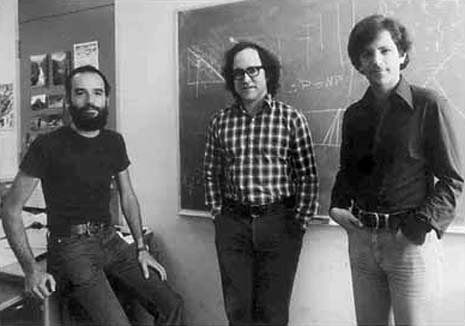
\includegraphics[width=0.5\textwidth]{img/rivest-shamir-adleman.jpg}
\end{center}
\end{frame}

%% Foto van links naar recht:
%% Adi Shamir, Ronald Rivest en Leonhard Adleman

\begin{frame}{RSA algoritme}
Alice wil een boodschap zenden naar Bob. 

\textbf{Enkel Bob} mag in staat zijn om de ciphertext terug om te zetten naar de plaintext.

De volgende stappen zijn nodig:

\begin{itemize}
	\item Bob genereert een publieke en private sleutel.
	\item Bob geeft de publieke sleutel aan Alice.
	\item Alice encrypteert de boodschap met de publieke sleutel van Bob.
	\item Bob gebruikt zijn private sleutel om de boodschap te decrypteren.
\end{itemize}

Opmerking: Eve beschikt \emph{niet}\/ over de private sleutel en kan de ciphertext 
m.a.w.\ niet ontcijferen.
\end{frame}

\begin{frame}{RSA Algoritme : Sleutelgeneratie}
\begin{itemize}
\item Bob kiest 2 grote priemgetallen (100 cijfers of meer). Laten we die getallen $p$ en $q$ noemen.
\item Bob berekent $n = p q$.	
\item Bob berekent $\varphi(n) = (p-1)(q-1)$. Bob kiest een getal $e$ dat geen factoren gemeenschappelijk heeft met $\varphi(n)$.
\item Bob bepaalt  de inverse modulo van $e$ module $\varphi(n)$. Dit getal noemen we $d$.
\end{itemize}

Bob's \textbf{publieke sleutel} is $(n, e)$.

\vspace{0.5cm}
Bob's \textbf{private sleutel} is $d$.  Deze private sleutel moet \textbf{geheim}
blijven.

\end{frame}

\begin{frame}{Priemgetallen?}
	Priemgetallen zijn de bouwstenen van alle andere getallen:  elk getal kan op een unieke manier gefactoriseerd worden in priemgetallen. 
	
	\vspace{0.5cm}
	Bv. 
	\[
		12 = 4 \times 3 = 2 \times 2 \times 3 = 2^2 \times 3
	\]
	
	\vspace{0.5cm}
	Er zijn \textbf{oneindig veel} priemgetallen.
\end{frame}

\begin{frame}{Wat is $\varphi(n)$?}

$\varphi(n)$ telt het aantal getallen tussen $1$ en $n-1$ die geen priemfactoren gemeenschappelijk
hebben met $n$; m.a.w.\ het aantal getallen $a$ tussen $1$ en $n-1$ waarvoor $\gcd(a, n) = 1$.

\vspace{0.5cm}
Beschouw $ n = 15$. Merk op dat $ 15 = 3 \times 5$.

Wat zijn de getallen die w\'el priemfactoren gemeenschappelijk hebben met $15$?
\[
3, 6 , 9, 12, 5, 10
\]
Dus 4 veelvouden van 3 en 2 veelvouden van 5: 
\[
15 - 1 - 4 - 2 = 8.
\]
In het algemeen: als $n = p q$:
\[
\varphi(n) = pq - 1 - (p-1) - (q-1) = (p-1)(q-1).
\]


\end{frame}


%	\begin{columns}
%		\begin{column}[T]{0.5\textwidth}
%		
%		\end{column}
%			\begin{column}[T]{0.5\textwidth}
%				Voorbeeld
%		\[ p_1 = 5 \wedge  p_2 = 7\]
%		\end{column}
%	\end{columns}

\begin{frame}{RSA Algoritme : Sleutelgeneratie}

\begin{itemize}
	\item Stel dat $p = 11$ en $q = 13$ worden gekozen.
	\item $ n = 11 \times 13 = 143$.
	\item $\varphi(n) = 10 \times 12 = 120$.
	\item Stel dat $e = 7$ wordt gekozen. (Dit is OK want $\gcd(120, 7) = 1$.
	\item We moeten de inverse van $e$ vinden modulo $120$. \\
	 Met het \textbf{uitgebreide algoritme van Euclides} vinden we dat $d = 103$.\\
	 Inderdaad $ 7 \times 103 = 721 = 6 \times 120 + 1$, en dus is 
	 $7 \times 103 \pmod{120} = 1$.
	  
\end{itemize}
\end{frame}

\begin{frame}{RSA Algoritme: Encryptie}
\begin{itemize}
	\item Alice wil een boodschap (plaintext) $m$ verzenden naar Bob. Alice gebruikt hiertoe de \textbf{publieke} sleutel $(n, e)$ van Bob.
	\item Alice berekent
	\[
	 c = m^e \pmod{n}.
	\]
	$c$ is de ciphertext die naar Bob wordt verstuurd.
	\item Merk op: de plaintext is m.a.w.\ een natuurlijk getal
	kleiner dan $n$.
\end{itemize}
\end{frame}

\begin{frame}{RSA Algoritme: Encryptie}
\begin{itemize}
	\item Alice wil de boodschap (plaintext) $m = 9$ verzenden naar Bob. 
	Alice gebruikt hiertoe de \textbf{publieke} sleutel $(n, e) = (143, 7)$ van Bob.
	\item Alice berekent
	\begin{align*}
	c & =  m^e \pmod{n} \\
	  & = 9^7 \pmod{143} \\
	  & = 9 \times 9^3 \times 9^3 \pmod{143} \\
	  & = 9\times 14\times 14 \\
	  &  = 1764 \pmod{143} \\
	  & =   48.
	\end{align*}
	$c$ is de ciphertext die naar Bob wordt verstuurd.
\end{itemize}
\end{frame}

\begin{frame}{RSA Algoritme: Decryptie}
\begin{itemize}
	\item Bob ontvangt de ciphertext $c$ van Alice. Hij gebruikt zijn \textbf{private} sleutel $d$ om deze te ontcijferen.
	\item Bob berekent
	\[
	c^d \pmod{n}.
	\]
	Dit zal steeds resulteren in de oorspronkelijke boodschap $m$!
\end{itemize}
\end{frame}


\begin{frame}{RSA Algoritme: Decryptie}
\begin{itemize}
	\item Bob ontvangt de ciphertext $c = 48$ van Alice. Hij gebruikt zijn \textbf{private} sleutel $d = 103$ om deze te ontcijferen.
	\item Bob berekent
	\begin{small}
	\begin{align*}
	c^d \pmod{n} & = 48^{103} \pmod{143} \\
	             & = 48 \times (48^{51})^2 \pmod{143} \\
	             & = 48 \times (48 \times (48^{25})^2)^2 \pmod{143} \\
	             & = 48 \times (48 \times ((48^5)^5)^2)^2 \pmod{143} \\ 
	             & = 48 \times (48 \times (133^5)^2)^2 \pmod{143} \\
	             & = 48 \times (48 \times (100)^2)^2 \pmod{143} \\  	           
	             & = 48 \times (48 \times 133)^2 \pmod{143} \\  
	             & = 48 \times (92)^2 \pmod{143} \\ 
	             & = 48 \times 27 \pmod{143} \\ 
	             & = 1296 \pmod{143} \\ 
	             & = 9 \pmod{143}.
	\end{align*}
	\end{small}
\end{itemize}
\end{frame}

%\begin{frame}{RSA Algoritme : stap 3}
%	\begin{columns}
%		\begin{column}[T]{0.5\textwidth}
%			Bereken een getal $\Phi$ =  het aantal getallen kleiner dan $m$ dat geen priemfactor met $m$ gemeenschappelijk heeft
%		\end{column}
%		\begin{column}[T]{0.5\textwidth}
%			Voorbeeld
%
%		\end{column}
%	\end{columns}	
%\end{frame}

%\begin{frame}{Priemfactoren?}
%	Priemgetallen zijn de bouwstenen van alle andere getallen:  elk getal kan opgedeeld worden in priemfactoren. 
%	
%	Bv. 
%	\[
%		12 = 4 \times 3 = 2 \times 2 \times 3 = 2^2 \times 3
%	\]
%	
%	
%\end{frame}

%\begin{frame}{RSA Algoritme : stap 3}
%	\begin{columns}
%		\begin{column}[T]{0.5\textwidth}
%			Bereken een getal $\Phi$ =  het aantal getallen kleiner dan $m$ dat geen priemfactor met $m$ gemeenschappelijk heeft
%		\end{column}
%		\begin{column}[T]{0.5\textwidth}
%			Voorbeeld
%			\[ p_1 = 5 \wedge  p_2 = 7\]
%			\[ 7 \times 5 = 35 = m \]
%			$m$ is opgebouwd uit de priemfactoren 5 en 7. Dus alle getallen onder de 35 waar een 5 of een 7 inzit vallen af.  Dat zijn 5, 10, 15, 20, 25, 30, 35, 7, 14, 21, 28  dus dat zijn er 11. Dus blijven er 35 - 11 = 24 getallen over, dus $\Phi$ = 24.
%		\end{column}
%	\end{columns}	
%\end{frame}

%\begin{frame}{RSA Algoritme : stap 3}
%	\begin{columns}
%		\begin{column}[T]{0.5\textwidth}
%			Bereken een getal $\Phi$ =  het aantal getallen kleiner dan $m$ dat geen priemfactor met $m$ gemeenschappelijk heeft
%		\end{column}
%		\begin{column}[T]{0.5\textwidth}
%			Voorbeeld
%			\[ p_1 = 5 \wedge  p_2 = 7\]
%			\[ 7 \times 5 = 35 = m \]
%			\[ \Phi = \Phi(p_1 . p_2) = (p_1 -1) \times (p_2 -1) \]
%		\end{column}
%	\end{columns}	
%\end{frame}

%\begin{frame}{RSA Algoritme : stap 3}
%	\begin{itemize}
%		\item Alle getallen uit de tafel van $p_1$  vallen af, dat zijn er $p_2$
%		\item Alle getallen uit de tafel van $p_2$ vallen af, dat zijn er $p_1$
%		\item Maar nu hebben we het getal $p_1 \times p_2$  dubbel meegeteld, dus er moet weer eentje bij.
%	\end{itemize}
%	
%	Dan blijft over  
%	\[ (p_1 \times p_2) - p_1 - p_2 + 1  =   (p_1 - 1)\times(p_2 - 1) \]
%\end{frame}

%\begin{frame}{RSA Algoritme : stap 3}
%	\begin{columns}
%		\begin{column}[T]{0.5\textwidth}
%			Bereken een getal $\Phi$ =  het aantal getallen kleiner dan $m$ dat geen priemfactor met $m$ gemeenschappelijk heeft
%		\end{column}
%		\begin{column}[T]{0.5\textwidth}
%			Voorbeeld
%			\[ p_1 = 5 \wedge  p_2 = 7\]
%			\[ 7 \times 5 = 35 = m \]
%			\[ \Phi(35) =4 \times 6 = 24 \]
%		\end{column}
%	\end{columns}	
%\end{frame}

%\begin{frame}{RSA Algoritme : stap 4}
%	\begin{columns}
%		\begin{column}[T]{0.5\textwidth}
%			Kies een nieuw getal $e$ kleiner $ < m$, waarvoor geldt dat dat getal geen deler met $\Phi$ gemeenschappelijk mag hebben.
%			
%			Dan is $e$  uit allemaal andere priemfactoren opgebouwd dan $\Phi$.
%		\end{column}
%		\begin{column}[T]{0.5\textwidth}
%			Voorbeeld
%			\[ p_1 = 5 \wedge  p_2 = 7\]
%			\[ 7 \times 5 = 35 = m \]
%			\[ \Phi(35) =4 \times 6 = 24 \]
%			\[ \Phi(35) =  2 . 2 . 2 . 3  \rightarrow e \in {5,7,25} \]  
%			Stel $e$ = 7.
%		\end{column}
%	\end{columns}	
%\end{frame}


%\begin{frame}{RSA Algoritme : stap 4}
%	\begin{columns}
%		\begin{column}[T]{0.5\textwidth}
%			Je maakt deze getallen  $m$ en $e$ openbaar. Zij vormen samen jouw publieke sleutel.
%		\end{column}
%		\begin{column}[T]{0.5\textwidth}
%			Voorbeeld
%			\[ p_1 = 5 \wedge  p_2 = 7\]
%			\[ 7 \times 5 = 35 = m \]
%			\[ \Phi(35) =4 \times 6 = 24 \]
%			\[ \Phi(35) =  2 . 2 . 2 . 3  \rightarrow e \in {5,7,25} \]  
%			Stel $e$ = 7. \\
%			Versleuteling is: \[ G = B^e  \pmod{m} \]
%		\end{column}
%	\end{columns}	
%\end{frame}

%\begin{frame}{RSA Algoritme : versleutelingsvoorbeeld}
%	\begin{itemize}
%		\item Stel A = 01, B = 02, C = 03 \dots.
%		\item Stel dat je het miniberichtje B = "12"  wilt versturen (de letter L dus). 
%		\item Dan bereken je dus  $G = 12^7 \pmod{35} = 33$
%		\item Je verstuurt  het geheime bericht $G = 33$.	
%	\end{itemize}
%\end{frame}
%
%\begin{frame}{RSA Algoritme : stap 5}
%	\begin{columns}
%		\begin{column}[T]{0.5\textwidth}
%			Cre\"eer $d$ waarvoor geldt:  $e \times d = 1 \pmod{\Phi}$.
%			Ontsleuteling is \[ B = 33^7 \pmod{35}  \]	
%	\end{column}
%		\begin{column}[T]{0.5\textwidth}
%			Voorbeeld
%			\[ B = 33^7 \pmod{35} \]
%			\[ 33^7 \pmod{35} \]
%			\[  33^4 \pmod{35} \times 33^3 \pmod{35} \]
%			\[ 51 \times 27 \pmod{35} \]
%			\[ 1377 \pmod{35} = 12 \]
%		\end{column}
%	\end{columns}	
%\end{frame}

\begin{frame}{Waarom werkt dit? Kleine stelling van Fermat}
De \textbf{kleine stelling van Fermat} zegt dat:
	Voor elk priemgetal $p$ en elk getal $a$ dat niet deelbaar is door $p$ geldt:  
	\[ a^{p-1} \pmod{p} = 1 \]
	
	Voorbeeld $a = 5$ en $p = 7$:  $5^6 = 15625 = 1 + 15624 = 1 + 7 \times 2232$, en dus
	\[
	5^6 \pmod{7} = 1 \pmod{7}
	\]
	
Meer algemeen geldt de \textbf{stelling van Euler}: 
Voor elke $a$ en $n$ met $\gcd(a,n) = 1$ geldt
\[
a^{\varphi(n)} \pmod{n} = 1.
\]
	
\end{frame}

\begin{frame}{Waarom werkt dit? }
\begin{itemize}
	\item 	Herinner je: de getallen $e$ en $d$ zijn zodanig gekozen dat $ e d \pmod{\varphi(n)} = 1$, ofte er bestaat een $k$ zodat
	\[
	ed = 1 + k \varphi(n)
	\]
	\item  $c = m^e\pmod{n}$, en wat Bob dus berekent bij het ontcijferen is
	\[
	c^d = (m^e \pmod{n})^d = m^{ed} \pmod{n}.
	\]	
	Nu geldt:
	\begin{align*}
	 m^{ed} \pmod{n} & = m^{1 + k\varphi(n)} \pmod{n} \\
	                 & = m ( m^{\varphi(n)})^k \pmod{n} \\
	                 & = m 1^k \pmod{n} \\
	                 & = m.
	\end{align*}
	(\tiny{Bewijs enkel geldig indien $\gcd(m, n) = 1$.})
\end{itemize}
\end{frame}

\begin{frame}{Waarom is dit moeilijk te kraken}
	\begin{itemize}
		\item RSA is zo moeilijk te ontcijferen omdat het haast niet te doen is om van een enorm getal $n$ te vinden uit welke twee priemgetallen $n$ is opgebouwd. Als $m$ uit veel meer priemfactoren zou bestaan zou dat veel makkelijker te vinden zijn, want zodra je er dan eentje hebt gevonden kun je m daardoor delen en wordt het snel kleiner.
		\item Verder is RSA ondanks die enorme getallen toch  makkelijk te gebruiken omdat machtsverheffen bij modulorekenen makkelijk is.
		\item 	Het bericht $m$ dat je wilt versturen mag niet groter zijn dan $n$. Als dat wel zo is, dan moet je het eerst in kleinere stukken hakken en die \'e\'en voor \'e\'en doorsturen.
	\end{itemize}


\end{frame}


\begin{frame}{RSA: Samenvatting}
	\begin{enumerate}
		\item Kies grote priemgetallen $p$ en $q$ (minstens 100 cijfers elk).
		\item Bepaal de modulus $n = p \times q$.
		\item Bereken $\varphi(n) = (p-1)(q-1)$.
		\item Kies een vercijferexponent $e$ waarvoor $\gcd(e,\varphi(n)) = 1$.
		\item Bereken $d$ zo, dat $e d  \pmod{\varphi(n)} = 1$.
		\item Maak de getallen $n$ en $e$ bekend. Samen vormen die de publieke sleutel.
		\item Houd $d$ geheim. Dat is de private sleutel.
		\item Vercijferen:$ E(m) = m^e \pmod{n}$
		\item Ontcijferen: $D(c) = c^d \pmod{n}$
	\end{enumerate}
\end{frame}

\begin{frame}{Voorbeeld}
\begin{itemize}
	 \pause\item Als priemgetallen nemen we $p = 74471$ en $q = 98773$. 
	 \pause\item De modulus $n = p \times q = 7355724083$.  Het getal $\varphi(n) = (p - 1)(q - 1) = 7355550840$.
	 \pause\item
	 Voor $e$ kiezen we $619$. Het (uitgebreide) algoritme van Euclides leert ons dat $\gcd(e,n) = 1$  en dat de inverse $d$ van $e$ modulo $\varphi(n)$ gelijk is aan $4313513659$.
	 \pause\item 
	  Neem nu als boodschap PRIEM. In cijfers wordt dat $m = 1618090513$. Vercijferen levert:
	  \[
	  c = 1618090513^{619} \pmod{7355724083} = 633613585
	  \]
	  \pause \item  Ontcijferen levert.
	  \[
	  c^d  \pmod{7355724083} = 1618090513
	  \]
	  \pause\item  We zien dat we inderdaad de originele boodschap terugvinden.
	  \end{itemize}
\end{frame}

\begin{frame}{Ontcijferen met verkeerde sleutel}
\begin{itemize}
	\item Stel dat we de boodschap proberen te ontcijferen met een willekeurige $d$, bv.\ $d = 12345678$.
	\item We vinden dan
	\[
	c^{12345678} \pmod{7355724083} = 1523535615
	\]
	\item We zien dat we een volledig andere boodschap krijgen!
\end{itemize}
\end{frame}


\begin{frame}{Wie is de verzender?}
\begin{itemize}
	\item Alice kan nu een boodschap verzenden naar Bob die enkel door Bob
	kan gelezen worden.
	\item Hoe kan Bob weten dat de boodschap van Alice afkomstig is 
	en niet van Eve?
	\pause \item Antwoord: dat is op dit moment \emph{niet}\/ mogelijk. Iedereen 
	kan een boodschap sturen naar Bob.
\end{itemize}
\end{frame}

\begin{frame}{Wie is de verzender?}
\begin{itemize}
	\item Hoe bewijst men in het \lq\lq echte\rq\rq\ leven wie de verzender is
	van een bepaalde boodschap/brief?
	\pause \item Men plaatst een handtekening.
	\pause \item De assumptie is dat enkel de \lq\lq echte\rq\rq\ persoon 
	in staat is de handtekening te plaatsen.
	\pause \item Alice moet m.a.w.\ iets doen wat door niemand anders kan 
	gedaan worden.
\end{itemize}	
\end{frame}

\begin{frame}{Wie is de verzender?}
\begin{itemize}
	\item Alice genereert een private $d_A$ en een publieke sleutel $(n_A, e_A)$. 
	\pause\item  Alice bezorgt de \textbf{publieke} sleutel aan Bob. (Op zo'n manier
	dat Bob zeker is dat de sleutel van Alice is.)
	\pause \item Wanneer Alice de boodschap $m$ naar Bob wil zenden dan
	  	ondertekent ze de boodschap met haar private sleutel:
	  	\[
	  	m_1 = m^{d_A} \pmod{n_A}.
	  	\]
	\pause \item Wanneer Bob de boodscahp $m_1$ ontvangt, dan kan hij 
	\textbf{verifi\"eren} dat de boodschap van Alice afkomstig is 
	door 
	\[
	m_1^{e_A} \pmod{n_A}
	\]
	te berekenen.
\end{itemize}
\end{frame}

\begin{frame}{Probleem ?}
\pause Iedereen kan de boodschap $m_1$ zien en iedereen met de publieke 
sleutel van Alice kan de boodschap lezen!

\vspace{0.5cm}
\pause Oplossing: pas encryptie toe op de getekende boodschap.
\begin{itemize}
	\item Alice wil $m$ verzenden naar Bob:
	\item Alice berekent $m_1 = m^d_A \pmod{n_A}$.
	\item Alice berekent vervolgens $c = m_1^{e_B} \pmod{n_B}$.
	\item Wanneer Bob de boodschap ontvangt dan gebruikt hij zijn private sleutel om $m_1$
	te berekenen:
	\[
	m_1 = c^{d_B} \pmod{n_B}
	\]
	\item Vervolgens gebruikt hij de publieke sleutel van Alice om de handtekening te verifi\"eren:
	\[
	m = m_1^{e_A} \pmod{n_A}.
	\]
\end{itemize}
\end{frame}


\begin{frame}{Zend elkaar een getekende en vercijferde boodschap}

Gebruik de Python-code om elkaar een getekende \'en vercijferde boodschap te verzenden.
\end{frame}





%---------- Back matter -------------------------------------------------------

\end{document}
